%\VignetteEngine{knitr::knitr}
%\VignetteIndexEntry{ELMER: Inferring Regulatory Element Landscapes and Transcription Factor Networks Using Methylomes}
% !Rnw weave = knitr
\documentclass{article}\usepackage[]{graphicx}\usepackage[usenames,dvipsnames]{color}
%% maxwidth is the original width if it is less than linewidth
%% otherwise use linewidth (to make sure the graphics do not exceed the margin)
\makeatletter
\def\maxwidth{ %
  \ifdim\Gin@nat@width>\linewidth
    \linewidth
  \else
    \Gin@nat@width
  \fi
}
\makeatother

\definecolor{fgcolor}{rgb}{0.345, 0.345, 0.345}
\newcommand{\hlnum}[1]{\textcolor[rgb]{0.686,0.059,0.569}{#1}}%
\newcommand{\hlstr}[1]{\textcolor[rgb]{0.192,0.494,0.8}{#1}}%
\newcommand{\hlcom}[1]{\textcolor[rgb]{0.678,0.584,0.686}{\textit{#1}}}%
\newcommand{\hlopt}[1]{\textcolor[rgb]{0,0,0}{#1}}%
\newcommand{\hlstd}[1]{\textcolor[rgb]{0.345,0.345,0.345}{#1}}%
\newcommand{\hlkwa}[1]{\textcolor[rgb]{0.161,0.373,0.58}{\textbf{#1}}}%
\newcommand{\hlkwb}[1]{\textcolor[rgb]{0.69,0.353,0.396}{#1}}%
\newcommand{\hlkwc}[1]{\textcolor[rgb]{0.333,0.667,0.333}{#1}}%
\newcommand{\hlkwd}[1]{\textcolor[rgb]{0.737,0.353,0.396}{\textbf{#1}}}%

\usepackage{framed}
\makeatletter
\newenvironment{kframe}{%
 \def\at@end@of@kframe{}%
 \ifinner\ifhmode%
  \def\at@end@of@kframe{\end{minipage}}%
  \begin{minipage}{\columnwidth}%
 \fi\fi%
 \def\FrameCommand##1{\hskip\@totalleftmargin \hskip-\fboxsep
 \colorbox{shadecolor}{##1}\hskip-\fboxsep
     % There is no \\@totalrightmargin, so:
     \hskip-\linewidth \hskip-\@totalleftmargin \hskip\columnwidth}%
 \MakeFramed {\advance\hsize-\width
   \@totalleftmargin\z@ \linewidth\hsize
   \@setminipage}}%
 {\par\unskip\endMakeFramed%
 \at@end@of@kframe}
\makeatother

\definecolor{shadecolor}{rgb}{.97, .97, .97}
\definecolor{messagecolor}{rgb}{0, 0, 0}
\definecolor{warningcolor}{rgb}{1, 0, 1}
\definecolor{errorcolor}{rgb}{1, 0, 0}
\newenvironment{knitrout}{}{} % an empty environment to be redefined in TeX

\usepackage{alltt}
\RequirePackage{/Library/Frameworks/R.framework/Versions/3.1/Resources/library/BiocStyle/resources/latex/Bioconductor}

\AtBeginDocument{\bibliographystyle{/Library/Frameworks/R.framework/Versions/3.1/Resources/library/BiocStyle/resources/latex/unsrturl}}

\usepackage[utf8]{inputenc}
\usepackage{graphicx}
\usepackage{grffile}
\usepackage{float}

\title{ELMER: An R/Bioconductor Tool \\
Inferring Regulatory Element Landscapes and Transcription Factor Networks Using Methylomes}
\author {Lijing Yao}
\IfFileExists{upquote.sty}{\usepackage{upquote}}{}
\begin{document}

\maketitle

\tableofcontents
\section{Introduction}
This document provides an introduction of the \Rpackage{ELMER}, which is designed 
to use DNA methylation and gene expression data sets from a large number
of tissue samples to infer regulatory element landscapes and transcription factor network.
It includes functions for identifying probes at distal regulatory regions with differential 
DNA methylation levels, predicting genes whose expression associates with the differentially
methylated probes and discovering the functional regulatory TFs. This package can be easily
applied to TCGA public available cancer data sets and to custom DNA methylation 
and gene expression data sets. 

\subsection{Installing and loading ELMER}
To obtain a copy of \Rpackage{ELMER}, you will need to install \Rpackage{devtools}
\begin{knitrout}
\definecolor{shadecolor}{rgb}{0.969, 0.969, 0.969}\color{fgcolor}\begin{kframe}
\begin{alltt}
\hlkwd{install.packages}\hlstd{(devtools)}
\hlkwd{library}\hlstd{(devtools);}
\hlstd{devtools}\hlopt{::}\hlkwd{install_github}\hlstd{(}\hlstr{"lijingya/ELMER"}\hlstd{);}
\end{alltt}
\end{kframe}
\end{knitrout}

\section{Download example data}
The following steps can be used to download the example data set for \Rpackage{ELMER}


\begin{knitrout}
\definecolor{shadecolor}{rgb}{0.969, 0.969, 0.969}\color{fgcolor}\begin{kframe}
\begin{alltt}
\hlcom{#Example file download from URL: https://dl.dropboxusercontent.com/u/61961845/ELMER.example.tar.gz}
\hlstd{URL} \hlkwb{<-} \hlstr{"https://dl.dropboxusercontent.com/u/61961845/ELMER.example.tar.gz"}
\hlkwd{download.file}\hlstd{(URL,}\hlkwc{destfile} \hlstd{=} \hlstr{"ELMER.example"}\hlstd{,}\hlkwc{method}\hlstd{=} \hlstr{"wget"}\hlstd{,}
              \hlkwc{extra} \hlstd{=} \hlkwd{c}\hlstd{(}\hlstr{"--no-check-certificate -a download.log"}\hlstd{))}
\hlkwd{untar}\hlstd{(}\hlstr{"./ELMER.example"}\hlstd{)}
\hlkwd{library}\hlstd{(ELMER)}
\end{alltt}
\end{kframe}
\end{knitrout}


\section{Quick start: running TCGA example}
Function, TCGA.pipe, is the easy usage for downloading TCGA data and performing all 
the analyses in ELMER. For illustration purpose, we skip the downloading step. 
The user can use the getTCGA function to download TCGA data or
use TCGA.pipe by including "download" in the analysis option.

\begin{knitrout}
\definecolor{shadecolor}{rgb}{0.969, 0.969, 0.969}\color{fgcolor}\begin{kframe}
\begin{alltt}
\hlkwd{TCGA.pipe}\hlstd{(}\hlstr{"LUSC"}\hlstd{,}\hlkwc{wd}\hlstd{=}\hlstr{"./ELMER.example"}\hlstd{,}\hlkwc{cores}\hlstd{=}\hlkwd{detectCores}\hlstd{()}\hlopt{/}\hlnum{2}\hlstd{,}\hlkwc{permu.size}\hlstd{=}\hlnum{300}\hlstd{,}
          \hlkwc{analysis} \hlstd{=} \hlkwd{c}\hlstd{(}\hlstr{"distal.enhancer"}\hlstd{,}\hlstr{"diffMeth"}\hlstd{,}\hlstr{"pair"}\hlstd{,}\hlstr{"motif"}\hlstd{,}\hlstr{"TF.search"}\hlstd{),}
          \hlkwc{diff.dir}\hlstd{=}\hlstr{"hypo"}\hlstd{,}\hlkwc{rm.chr}\hlstd{=}\hlkwd{paste0}\hlstd{(}\hlstr{"chr"}\hlstd{,}\hlkwd{c}\hlstd{(}\hlnum{1}\hlopt{:}\hlnum{22}\hlstd{,}\hlstr{"X"}\hlstd{,}\hlstr{"Y"}\hlstd{)))}
\end{alltt}


{\ttfamily\noindent\itshape\color{messagecolor}{\#\# \#\#\#\#\#\#\#\#\#\#\#\#\#\#\#\#\#\#\#\\\#\# Select distal enhancer probes\\\#\# \#\#\#\#\#\#\#\#\#\#\#\#\#\#\#\#\#\#\#}}

{\ttfamily\noindent\color{warningcolor}{\#\# Warning in (function (probe, distal = TRUE, feature, TSS, TSS.range = list(upstream = 2000, : Default probes coordinates are for HM450K DNA methylation array}}

{\ttfamily\noindent\itshape\color{messagecolor}{\#\# \#\#\#\#\#\#\#\#\#\#\#\#\#\#\#\#\#\#\#\\\#\# Get differential DNA methylation loci\\\#\# \#\#\#\#\#\#\#\#\#\#\#\#\#\#\#\#\#\#\#\\\#\# \\\#\# \\\#\# \textasciitilde{}\textasciitilde{}\textasciitilde{} MEE.data: initializator \textasciitilde{}\textasciitilde{}\textasciitilde{} \\\#\# \#\#\#\#\#\#\#\#\#\#\#\#\#\#\#\#\#\#\#\\\#\# Predict pairs\\\#\# \#\#\#\#\#\#\#\#\#\#\#\#\#\#\#\#\#\#\#\\\#\# \\\#\# \\\#\# \textasciitilde{}\textasciitilde{}\textasciitilde{} MEE.data: initializator \textasciitilde{}\textasciitilde{}\textasciitilde{} \\\#\# Identify putative probe-gene pair for hypomethylated probes\\\#\# Calculate empirical P value.\\\#\# \\\#\# \#\#\#\#\#\#\#\#\#\#\#\#\#\#\#\#\#\#\#\\\#\# Motif search\\\#\# \#\#\#\#\#\#\#\#\#\#\#\#\#\#\#\#\#\#\#\\\#\# \\\#\# \\\#\# Identify enriched motif for hypomethylated probes\\\#\# 12 motifs are enriched.\\\#\# \#\#\#\#\#\#\#\#\#\#\#\#\#\#\#\#\#\#\#\\\#\# Search responsible TFs\\\#\# \#\#\#\#\#\#\#\#\#\#\#\#\#\#\#\#\#\#\#\\\#\# \\\#\# \\\#\# \textasciitilde{}\textasciitilde{}\textasciitilde{} MEE.data: initializator \textasciitilde{}\textasciitilde{}\textasciitilde{} \\\#\# Identify regulatory TF for enriched motif in hypomethylated probes}}\end{kframe}
\end{knitrout}


\section{Input data}

The whole pipeline analyses in \Rpackage{ELMER} needs at least 4 input files:
a matrix of DNA methylation from HM450K platform; a matrix of gene expression for the 
same samples; a GRanges object containing the information for probes on HM450K such as names 
and coordinates; a gene annotation which is also a GRanges object. When TCGA data are used,
the sample information will be automatically generated by fetch.mee function. However
sample information should be provided when using custom data.

\subsection{DNA methylation data}
Raw DNA methylation data can be processed by \Rpackage{Methylumi} or \Rpackage{minfi}
generating DNA methylation information for each CpG. The DNA methylation level 
at each CpG is referred to as a beta ($\beta$) value, calculated as (M/(M+U)), 
where M represents the methylated allele intensity and U the unmethylated allele 
intensity. Beta values range from 0 to 1, reflecting the fraction of methylated 
alleles at each CpG in the each tumor; beta values close to 0 indicates low 
levels of DNA methylation and beta values close to 1 indicates high levels 
of DNA methylation. Generate a matrix with DNA methylation beta values for all
the samples (columns) and probe loci (rows) and save matrix as meth.rda

\begin{knitrout}
\definecolor{shadecolor}{rgb}{0.969, 0.969, 0.969}\color{fgcolor}\begin{kframe}
\begin{alltt}
\hlkwd{load}\hlstd{(}\hlstr{"./ELMER.example/Result/LUSC/LUSC_meth_refined.rda"}\hlstd{)}
\hlstd{Meth[}\hlnum{1}\hlopt{:}\hlnum{10}\hlstd{,} \hlnum{1}\hlopt{:}\hlnum{2}\hlstd{]}
\end{alltt}
\begin{verbatim}
##            TCGA-43-3394-11A-01D-1551-05 TCGA-43-3920-11B-01D-1551-05
## cg00045114                    0.8190894                    0.8073763
## cg00050294                    0.8423084                    0.8241138
## cg00066722                    0.9101127                    0.9162212
## cg00093522                    0.8751903                    0.8864599
## cg00107046                    0.3326016                    0.3445508
## cg00116430                    0.6097183                    0.5952469
## cg00152117                    0.7074149                    0.6439695
## cg00163018                    0.5928909                    0.8250584
## cg00173804                    0.9162264                    0.9303684
## cg00223046                    0.7826863                    0.7744760
\end{verbatim}
\end{kframe}
\end{knitrout}

\subsection{Gene expression data}
Gene expression values can be generated from different platforms such as array or 
RNA-seq, gene level or transcript level gene expression calling. Generate a matrix 
with gene expression values for all the samples (columns) and genes (rows) 
and save matrix as RNA.rda

\begin{knitrout}
\definecolor{shadecolor}{rgb}{0.969, 0.969, 0.969}\color{fgcolor}\begin{kframe}
\begin{alltt}
\hlkwd{load}\hlstd{(}\hlstr{"./ELMER.example/Result/LUSC/LUSC_RNA_refined.rda"}\hlstd{)}
\hlstd{GeneExp[}\hlnum{1}\hlopt{:}\hlnum{10}\hlstd{,} \hlnum{1}\hlopt{:}\hlnum{2}\hlstd{]}
\end{alltt}
\begin{verbatim}
##          TCGA-22-5472-01A-01R-1635-07 TCGA-22-5489-01A-01R-1635-07
## ID126767                    0.0000000                     0.000000
## ID343066                    0.4303923                     0.000000
## ID26574                    10.0817831                    10.717673
## ID24                        6.4462711                     6.386644
## ID23456                     8.5929182                     9.333097
## ID5825                     10.5578756                     9.878333
## ID25                       10.7233258                    11.075515
## ID27                        8.9761542                     9.569239
## ID29777                     9.6415206                     9.353424
## ID80325                     8.9840983                     9.177624
\end{verbatim}
\end{kframe}
\end{knitrout}


\subsection{Sample information}
Sample information should be stored as a data.frame object containing sample ID, 
group labels (such as tumor, normal) and other description for each sample. 
When TCGA data were used, tumor, normal group label will be automatically generated by 
fetch.mee function by specifying option TCGA=TRUE.

\begin{knitrout}
\definecolor{shadecolor}{rgb}{0.969, 0.969, 0.969}\color{fgcolor}\begin{kframe}
\begin{alltt}
\hlstd{mee} \hlkwb{<-} \hlkwd{fetch.mee}\hlstd{(}\hlkwc{meth}\hlstd{=Meth,} \hlkwc{exp}\hlstd{=GeneExp,} \hlkwc{TCGA}\hlstd{=T)}
\end{alltt}


{\ttfamily\noindent\itshape\color{messagecolor}{\#\# \textasciitilde{}\textasciitilde{}\textasciitilde{} MEE.data: initializator \textasciitilde{}\textasciitilde{}\textasciitilde{}}}\begin{alltt}
\hlkwd{head}\hlstd{(}\hlkwd{getSample}\hlstd{(mee))}
\end{alltt}
\begin{verbatim}
##                              ID                      meth.ID                       exp.ID
## TCGA-43-3394-11 TCGA-43-3394-11 TCGA-43-3394-11A-01D-1551-05 TCGA-43-3394-11A-01R-1758-07
## TCGA-56-8305-01 TCGA-56-8305-01 TCGA-56-8305-01A-11D-2294-05 TCGA-56-8305-01A-11R-2296-07
## TCGA-56-8307-01 TCGA-56-8307-01 TCGA-56-8307-01A-11D-2294-05 TCGA-56-8307-01A-11R-2296-07
## TCGA-56-8308-01 TCGA-56-8308-01 TCGA-56-8308-01A-11D-2294-05 TCGA-56-8308-01A-11R-2296-07
## TCGA-56-8309-01 TCGA-56-8309-01 TCGA-56-8309-01A-11D-2294-05 TCGA-56-8309-01A-11R-2296-07
## TCGA-58-8386-01 TCGA-58-8386-01 TCGA-58-8386-01A-11D-2294-05 TCGA-58-8386-01A-11R-2296-07
##                     TN
## TCGA-43-3394-11 Normal
## TCGA-56-8305-01  Tumor
## TCGA-56-8307-01  Tumor
## TCGA-56-8308-01  Tumor
## TCGA-56-8309-01  Tumor
## TCGA-58-8386-01  Tumor
\end{verbatim}
\end{kframe}
\end{knitrout}

\subsection{Probe information}
Probe information should be stored as a GRanges object containing the coordinate 
of each probe on the DNA methylation array and names of each probe. 
The default probe information is for HM450K. 

\begin{knitrout}
\definecolor{shadecolor}{rgb}{0.969, 0.969, 0.969}\color{fgcolor}\begin{kframe}
\begin{alltt}
\hlstd{probe} \hlkwb{<-} \hlkwd{ReadBed}\hlstd{(}\hlkwd{system.file}\hlstd{(}\hlstr{"extdata"}\hlstd{,}\hlstr{"Illumina-methyl-450K-manifest.hg19.bed.xz"}\hlstd{,}
                             \hlkwc{package} \hlstd{=} \hlstr{"ELMER"}\hlstd{))}
\hlstd{mee} \hlkwb{<-} \hlkwd{fetch.mee}\hlstd{(}\hlkwc{meth}\hlstd{=Meth,} \hlkwc{exp}\hlstd{=GeneExp,} \hlkwc{TCGA}\hlstd{=T,} \hlkwc{probeInfo}\hlstd{=probe)}
\end{alltt}


{\ttfamily\noindent\itshape\color{messagecolor}{\#\# \textasciitilde{}\textasciitilde{}\textasciitilde{} MEE.data: initializator \textasciitilde{}\textasciitilde{}\textasciitilde{}}}\begin{alltt}
\hlkwd{getProbeInfo}\hlstd{(mee)}
\end{alltt}
\begin{verbatim}
## GRanges object with 1725 ranges and 1 metadata column:
##          seqnames                 ranges strand   |            name
##             <Rle>              <IRanges>  <Rle>   |     <character>
##      [1]     chr1 [172674159, 172674159]      *   |      cg00045114
##      [2]     chr1 [  2886818,   2886818]      *   |      cg00050294
##      [3]     chr1 [ 43634520,  43634520]      *   |      cg00066722
##      [4]     chr1 [  2252019,   2252019]      *   |      cg00093522
##      [5]     chr1 [ 16465562,  16465562]      *   |      cg00107046
##      ...      ...                    ...    ... ...             ...
##   [1721]     chr1 [215147891, 215147891]      *   |      cg27589988
##   [1722]     chr1 [ 46632696,  46632696]      *   |      cg27636310
##   [1723]     chr1 [  3472204,   3472204]      *   |      cg27637706
##   [1724]     chr1 [  3283394,   3283394]      *   |    ch.1.131529R
##   [1725]     chr1 [174947362, 174947362]      *   | ch.1.173213985R
##   -------
##   seqinfo: 24 sequences from an unspecified genome; no seqlengths
\end{verbatim}
\end{kframe}
\end{knitrout}

\subsection{Gene information}
Gene information should be stored as a GRanges object containing coordinates of 
each gene, gene id, gene symbol and gene isoform id. The default gene information 
is the UCSC gene annotation. 


\begin{knitrout}
\definecolor{shadecolor}{rgb}{0.969, 0.969, 0.969}\color{fgcolor}\begin{kframe}
\begin{alltt}
\hlkwd{load}\hlstd{(}\hlkwd{system.file}\hlstd{(}\hlstr{"extdata"}\hlstd{,}\hlstr{"UCSC_gene_hg19.rda"}\hlstd{,}\hlkwc{package} \hlstd{=} \hlstr{"ELMER"}\hlstd{))}
\hlcom{## In TCGA expression data, geneIDs were used as the rowname for each row. However, numbers }
\hlcom{## can't be the rownames, "ID" was added to each gene id functioning as the rowname.}
\hlcom{## If your geneID is consistent with the rownames of the gene expression matrix, adding "ID" }
\hlcom{## to each geneID can be skipped.}
\hlstd{txs}\hlopt{$}\hlstd{GENEID} \hlkwb{<-} \hlkwd{paste0}\hlstd{(}\hlstr{"ID"}\hlstd{,txs}\hlopt{$}\hlstd{GENEID)}
\hlstd{geneInfo} \hlkwb{<-} \hlkwd{promoters}\hlstd{(txs,}\hlkwc{upstream} \hlstd{=} \hlnum{0}\hlstd{,} \hlkwc{downstream} \hlstd{=} \hlnum{0}\hlstd{)}
\hlkwd{save}\hlstd{(geneInfo,}\hlkwc{file}\hlstd{=}\hlstr{"./ELMER.example/Result/LUSC/geneAnnot.rda"}\hlstd{)}
\hlstd{mee} \hlkwb{<-} \hlkwd{fetch.mee}\hlstd{(}\hlkwc{meth}\hlstd{=Meth,} \hlkwc{exp}\hlstd{=GeneExp,} \hlkwc{TCGA}\hlstd{=T,} \hlkwc{geneInfo}\hlstd{=txs)}
\end{alltt}


{\ttfamily\noindent\itshape\color{messagecolor}{\#\# \textasciitilde{}\textasciitilde{}\textasciitilde{} MEE.data: initializator \textasciitilde{}\textasciitilde{}\textasciitilde{}}}\begin{alltt}
\hlkwd{getGeneInfo}\hlstd{(mee)}
\end{alltt}
\begin{verbatim}
## GRanges object with 13741 ranges and 3 metadata columns:
##         seqnames                 ranges strand   |     tx_name      GENEID      SYMBOL
##            <Rle>              <IRanges>  <Rle>   | <character> <character> <character>
##   10000     chr1 [243651535, 244006584]      -   |  uc001hzz.1     ID10000        AKT3
##   10000     chr1 [243663021, 244006584]      -   |  uc001iab.2     ID10000        AKT3
##   10000     chr1 [243663021, 244006886]      -   |  uc021plu.1     ID10000        AKT3
##   10001    chr14 [ 71050957,  71067384]      -   |  uc001xmf.3     ID10001        MED6
##   10001    chr14 [ 71050957,  71067384]      -   |  uc010tth.2     ID10001        MED6
##     ...      ...                    ...    ... ...         ...         ...         ...
##    9988     chr7   [86781677, 86825648]      +   |  uc003uik.3      ID9988       DMTF1
##    9988     chr7   [86781677, 86825648]      +   |  uc011khb.2      ID9988       DMTF1
##    9988     chr7   [86781870, 86825648]      +   |  uc003uil.3      ID9988       DMTF1
##    9988     chr7   [86792198, 86809018]      +   |  uc003uim.1      ID9988       DMTF1
##    9988     chr7   [86792198, 86825648]      +   |  uc003uin.3      ID9988       DMTF1
##   -------
##   seqinfo: 93 sequences (1 circular) from hg19 genome
\end{verbatim}
\end{kframe}
\end{knitrout}

\subsection{MEE.data}
The above 5 components will generate a MEE.data object as the main input for mulitple functions 
in \Rpackage{ELMER}.

\begin{knitrout}
\definecolor{shadecolor}{rgb}{0.969, 0.969, 0.969}\color{fgcolor}\begin{kframe}
\begin{alltt}
\hlstd{mee} \hlkwb{<-} \hlkwd{fetch.mee}\hlstd{(}\hlkwc{meth}\hlstd{=Meth,} \hlkwc{exp}\hlstd{=GeneExp,} \hlkwc{TCGA}\hlstd{=T,} \hlkwc{probeInfo}\hlstd{=probe,} \hlkwc{geneInfo}\hlstd{=txs)}
\end{alltt}


{\ttfamily\noindent\itshape\color{messagecolor}{\#\# \textasciitilde{}\textasciitilde{}\textasciitilde{} MEE.data: initializator \textasciitilde{}\textasciitilde{}\textasciitilde{}}}\begin{alltt}
\hlstd{mee}
\end{alltt}
\begin{verbatim}
## *** Class MEE.data, method show *** 
## * meth 
##  num [1:1725, 1:234] 0.819 0.842 0.91 0.875 0.333 ...
##  - attr(*, "dimnames")=List of 2
##   ..$ : chr [1:1725] "cg00045114" "cg00050294" "cg00066722" "cg00093522" ...
##   ..$ : chr [1:234] "TCGA-43-3394-11A-01D-1551-05" "TCGA-56-8305-01A-11D-2294-05" "TCGA-56-8307-01A-11D-2294-05" "TCGA-56-8308-01A-11D-2294-05" ...
## NULL
## * exp 
##  num [1:3894, 1:234] 0 0.214 10.048 5.007 8.63 ...
##  - attr(*, "dimnames")=List of 2
##   ..$ : chr [1:3894] "ID126767" "ID343066" "ID26574" "ID24" ...
##   ..$ : chr [1:234] "TCGA-43-3394-11A-01R-1758-07" "TCGA-56-8305-01A-11R-2296-07" "TCGA-56-8307-01A-11R-2296-07" "TCGA-56-8308-01A-11R-2296-07" ...
## NULL
## * sample 
## 'data.frame':	234 obs. of  4 variables:
##  $ ID     : chr  "TCGA-43-3394-11" "TCGA-56-8305-01" "TCGA-56-8307-01" "TCGA-56-8308-01" ...
##  $ meth.ID: chr  "TCGA-43-3394-11A-01D-1551-05" "TCGA-56-8305-01A-11D-2294-05" "TCGA-56-8307-01A-11D-2294-05" "TCGA-56-8308-01A-11D-2294-05" ...
##  $ exp.ID : chr  "TCGA-43-3394-11A-01R-1758-07" "TCGA-56-8305-01A-11R-2296-07" "TCGA-56-8307-01A-11R-2296-07" "TCGA-56-8308-01A-11R-2296-07" ...
##  $ TN     : chr  "Normal" "Tumor" "Tumor" "Tumor" ...
## NULL
## * probeInfo 
## GRanges object with 1725 ranges and 1 metadata column:
##          seqnames                 ranges strand   |            name
##             <Rle>              <IRanges>  <Rle>   |     <character>
##      [1]     chr1 [172674159, 172674159]      *   |      cg00045114
##      [2]     chr1 [  2886818,   2886818]      *   |      cg00050294
##      [3]     chr1 [ 43634520,  43634520]      *   |      cg00066722
##      [4]     chr1 [  2252019,   2252019]      *   |      cg00093522
##      [5]     chr1 [ 16465562,  16465562]      *   |      cg00107046
##      ...      ...                    ...    ... ...             ...
##   [1721]     chr1 [215147891, 215147891]      *   |      cg27589988
##   [1722]     chr1 [ 46632696,  46632696]      *   |      cg27636310
##   [1723]     chr1 [  3472204,   3472204]      *   |      cg27637706
##   [1724]     chr1 [  3283394,   3283394]      *   |    ch.1.131529R
##   [1725]     chr1 [174947362, 174947362]      *   | ch.1.173213985R
##   -------
##   seqinfo: 24 sequences from an unspecified genome; no seqlengths
## * geneInfo 
## GRanges object with 13741 ranges and 3 metadata columns:
##         seqnames                 ranges strand   |     tx_name      GENEID      SYMBOL
##            <Rle>              <IRanges>  <Rle>   | <character> <character> <character>
##   10000     chr1 [243651535, 244006584]      -   |  uc001hzz.1     ID10000        AKT3
##   10000     chr1 [243663021, 244006584]      -   |  uc001iab.2     ID10000        AKT3
##   10000     chr1 [243663021, 244006886]      -   |  uc021plu.1     ID10000        AKT3
##   10001    chr14 [ 71050957,  71067384]      -   |  uc001xmf.3     ID10001        MED6
##   10001    chr14 [ 71050957,  71067384]      -   |  uc010tth.2     ID10001        MED6
##     ...      ...                    ...    ... ...         ...         ...         ...
##    9988     chr7   [86781677, 86825648]      +   |  uc003uik.3      ID9988       DMTF1
##    9988     chr7   [86781677, 86825648]      +   |  uc011khb.2      ID9988       DMTF1
##    9988     chr7   [86781870, 86825648]      +   |  uc003uil.3      ID9988       DMTF1
##    9988     chr7   [86792198, 86809018]      +   |  uc003uim.1      ID9988       DMTF1
##    9988     chr7   [86792198, 86825648]      +   |  uc003uin.3      ID9988       DMTF1
##   -------
##   seqinfo: 93 sequences (1 circular) from hg19 genome
## ******* End Print (MEE.data) *******
\end{verbatim}
\end{kframe}
\end{knitrout}

\section{Illustration of ELMER analysis steps}
A subset of chromosome 1 data from TCGA LUSC were used as illustruation. 

\subsection{Selection of probes within biofeatures}
Function, get.feature.probe, is used to select probes that are located within 
biofeatures such as H3K27ac ChIP-seq peaks. As default, the get.feature.probe function
will automatically select distal enhancer probes on HM450K which are at least 
2kb away from the TSS annotated by GENCODE V15 and UCSC-gene and locate within 
the putative comprehensive enhancers from REMC, ENCODE and FANTOM5. 
\begin{knitrout}
\definecolor{shadecolor}{rgb}{0.969, 0.969, 0.969}\color{fgcolor}\begin{kframe}
\begin{alltt}
\hlcom{#get distal enhancer probes that are 2kb away from TSS and overlap with REMC and FANTOM5 }
\hlcom{#enhancers on chromosome 1}
\hlstd{Probe} \hlkwb{<-} \hlkwd{get.feature.probe}\hlstd{(}\hlkwc{probe}\hlstd{=probe,} \hlkwc{rm.chr}\hlstd{=}\hlkwd{paste0}\hlstd{(}\hlstr{"chr"}\hlstd{,}\hlkwd{c}\hlstd{(}\hlnum{2}\hlopt{:}\hlnum{22}\hlstd{,}\hlstr{"X"}\hlstd{,}\hlstr{"Y"}\hlstd{)))}
\hlkwd{save}\hlstd{(Probe,}\hlkwc{file}\hlstd{=}\hlstr{"./ELMER.example/Result/LUSC/probeInfo_feature.rda"}\hlstd{)}
\end{alltt}
\end{kframe}
\end{knitrout}


\subsection{Identifying differentially methylated probes}
Function, get.diff.meth, will be used to identify differentially methylated 
probes among the ones within biofeatures, which are selected in the above step. 
\begin{knitrout}
\definecolor{shadecolor}{rgb}{0.969, 0.969, 0.969}\color{fgcolor}\begin{kframe}
\begin{alltt}
\hlcom{## fetch.mee can take path as input.}
\hlstd{mee} \hlkwb{<-} \hlkwd{fetch.mee}\hlstd{(}\hlkwc{meth}\hlstd{=}\hlstr{"./ELMER.example/Result/LUSC/LUSC_meth_refined.rda"}\hlstd{,}
                 \hlkwc{exp}\hlstd{=}\hlstr{"./ELMER.example/Result/LUSC/LUSC_RNA_refined.rda"}\hlstd{,} \hlkwc{TCGA}\hlstd{=T,}
                 \hlkwc{probeInfo}\hlstd{=}\hlstr{"./ELMER.example/Result/LUSC/probeInfo_feature.rda"}\hlstd{,}
                 \hlkwc{geneInfo}\hlstd{=}\hlstr{"./ELMER.example/Result/LUSC/geneAnnot.rda"}\hlstd{)}
\end{alltt}


{\ttfamily\noindent\itshape\color{messagecolor}{\#\# \textasciitilde{}\textasciitilde{}\textasciitilde{} MEE.data: initializator \textasciitilde{}\textasciitilde{}\textasciitilde{}}}\begin{alltt}
\hlstd{sig.diff} \hlkwb{<-} \hlkwd{get.diff.meth}\hlstd{(mee,} \hlkwc{cores}\hlstd{=}\hlkwd{detectCores}\hlstd{()}\hlopt{/}\hlnum{2}\hlstd{,} \hlkwc{dir.out} \hlstd{=}\hlstr{"./ELMER.example/Result/LUSC"}\hlstd{,}
                          \hlkwc{diff.dir}\hlstd{=}\hlstr{"hypo"}\hlstd{,} \hlkwc{pvalue} \hlstd{=} \hlnum{0.01}\hlstd{)}

\hlstd{sig.diff}\hlopt{$}\hlstd{hypo[}\hlnum{1}\hlopt{:}\hlnum{10}\hlstd{,]}   \hlcom{## significantly hypomethylated probes}
\end{alltt}
\begin{verbatim}
##                 probe       pvalue tumorMinNormal     adjust.p
## cg00045114 cg00045114 7.307478e-13     -0.3499588 2.419463e-12
## cg00050294 cg00050294 4.440329e-09     -0.5000920 1.057951e-08
## cg00093522 cg00093522 1.143338e-23     -0.3596944 1.001147e-22
## cg00163018 cg00163018 2.240026e-21     -0.3838195 1.558083e-20
## cg00173804 cg00173804 2.767232e-18     -0.3744557 1.455328e-17
## cg00223046 cg00223046 8.142751e-11     -0.3313773 2.317862e-10
## cg00255699 cg00255699 6.386989e-13     -0.4308994 2.126941e-12
## cg00292636 cg00292636 6.368018e-34     -0.4833375 2.112468e-32
## cg00329272 cg00329272 6.864176e-39     -0.4355332 5.638431e-37
## cg00340127 cg00340127 3.056522e-18     -0.5857140 1.602584e-17
\end{verbatim}
\begin{alltt}
\hlcom{# get.diff.meth automatically save output files. }
\hlcom{# getMethdiff.hypo.probes.csv contains statistics for all the probes.}
\hlcom{# getMethdiff.hypo.probes.significant.csv contains only the significant probes.}
\hlkwd{dir}\hlstd{(}\hlkwc{path} \hlstd{=} \hlstr{"./ELMER.example/Result/LUSC"}\hlstd{,} \hlkwc{pattern} \hlstd{=} \hlstr{"getMethdiff"}\hlstd{)}
\end{alltt}
\begin{verbatim}
## [1] "getMethdiff.hypo.probes.csv"             "getMethdiff.hypo.probes.significant.csv"
\end{verbatim}
\end{kframe}
\end{knitrout}


\subsection{Identifying putative probe-gene pairs}
Function, get.pair function, will be used to identify putative target genes for selected probes. 
This step is the most time consuming step since it requires a large amount calculations 
for permutation. The greater the permutation time is, the longer it will take. 
It is recommended to use multiple cores for this step. Default permutation time 
is 1000 which may need 12 hrs by 4 cores. However 10,000 permutations is recommended 
which may cost 2 days, if high confidence results are desired.
\begin{knitrout}
\definecolor{shadecolor}{rgb}{0.969, 0.969, 0.969}\color{fgcolor}\begin{kframe}
\begin{alltt}
\hlcom{### identify target gene for significantly hypomethylated probes.}

\hlstd{Sig.probes} \hlkwb{<-} \hlkwd{read.csv}\hlstd{(}\hlstr{"./ELMER.example/Result/LUSC/getMethdiff.hypo.probes.significant.csv"}\hlstd{,}
                       \hlkwc{stringsAsFactors}\hlstd{=F)[,}\hlnum{1}\hlstd{]}
\hlkwd{head}\hlstd{(Sig.probes)}  \hlcom{# significantly hypomethylated probes}
\end{alltt}
\begin{verbatim}
## [1] "cg00045114" "cg00050294" "cg00093522" "cg00163018" "cg00173804" "cg00223046"
\end{verbatim}
\begin{alltt}
\hlcom{## Collect nearby 20 gene for Sig.probes}
\hlstd{nearGenes} \hlkwb{<-}\hlkwd{GetNearGenes}\hlstd{(}\hlkwc{TRange}\hlstd{=}\hlkwd{getProbeInfo}\hlstd{(mee,}\hlkwc{probe}\hlstd{=Sig.probes),}
                         \hlkwc{geneAnnot}\hlstd{=}\hlkwd{getGeneInfo}\hlstd{(mee),}\hlkwc{cores}\hlstd{=}\hlkwd{detectCores}\hlstd{()}\hlopt{/}\hlnum{2}\hlstd{)}

\hlcom{## Identify significant probe-gene pairs}
\hlstd{Hypo.pair} \hlkwb{<-}\hlkwd{get.pair}\hlstd{(}\hlkwc{mee}\hlstd{=mee,}\hlkwc{probes}\hlstd{=Sig.probes,}\hlkwc{nearGenes}\hlstd{=nearGenes,}
                     \hlkwc{permu.dir}\hlstd{=}\hlstr{"./ELMER.example/Result/LUSC/permu"}\hlstd{,}\hlkwc{permu.size}\hlstd{=}\hlnum{300}\hlstd{,}\hlkwc{Pe} \hlstd{=} \hlnum{0.01}\hlstd{,}
                     \hlkwc{dir.out}\hlstd{=}\hlstr{"./ELMER.example/Result/LUSC"}\hlstd{,}\hlkwc{cores}\hlstd{=}\hlkwd{detectCores}\hlstd{()}\hlopt{/}\hlnum{2}\hlstd{,}\hlkwc{label}\hlstd{=} \hlstr{"hypo"}\hlstd{)}
\end{alltt}


{\ttfamily\noindent\itshape\color{messagecolor}{\#\# Calculate empirical P value.}}\begin{alltt}
\hlkwd{head}\hlstd{(Hypo.pair)}  \hlcom{## significant probe-gene pairs}
\end{alltt}
\begin{verbatim}
##                          Probe   GeneID   Symbol Distance Sides        Raw.p          Pe
## cg20701183.ID8543   cg20701183   ID8543     LMO4     2563    L1 7.453984e-14 0.003322259
## cg19403323.ID255928 cg19403323 ID255928    SYT14    87477    R1 1.671937e-12 0.003322259
## cg12213388.ID84451  cg12213388  ID84451 KIAA1804   993548    L4 2.527644e-12 0.003322259
## cg26607897.ID55811  cg26607897  ID55811   ADCY10   292476    R3 4.593610e-12 0.003322259
## cg10574861.ID8543   cg10574861   ID8543     LMO4     4715    L1 4.770162e-12 0.003322259
## cg26607897.ID23432  cg26607897  ID23432   GPR161   563308    R6 8.048248e-12 0.003322259
\end{verbatim}
\begin{alltt}
\hlcom{# get.pair automatically save output files. }
\hlcom{#getPair.hypo.all.pairs.statistic.csv contains statistics for all the probe-gene pairs.}
\hlcom{#getPair.hypo.pairs.significant.csv contains only the significant probes.}
\hlkwd{dir}\hlstd{(}\hlkwc{path} \hlstd{=} \hlstr{"./ELMER.example/Result/LUSC"}\hlstd{,} \hlkwc{pattern} \hlstd{=} \hlstr{"getPair"}\hlstd{)}
\end{alltt}
\begin{verbatim}
## [1] "getPair.hypo.all.pairs.statistic.csv"        
## [2] "getPair.hypo.pairs.significant.csv"          
## [3] "getPair.hypo.pairs.significant.withmotif.csv"
\end{verbatim}
\end{kframe}
\end{knitrout}


\subsection{Motif enrichment analysis on the selected probes}
Function, get.enriched.motif, will be used to calculate enrichment of the motifs from 
factorbook and JASPER for the selected probes. Odds Ratio is used to assess 
the enrichment levels and 95\% confidence interval of Odds Ratio is calculated.
\begin{knitrout}
\definecolor{shadecolor}{rgb}{0.969, 0.969, 0.969}\color{fgcolor}\begin{kframe}
\begin{alltt}
\hlcom{### identify enriched motif for significantly hypomethylated probes which }
\hlcom{##have putative target genes.}

\hlstd{Sig.probes.paired} \hlkwb{<-} \hlkwd{read.csv}\hlstd{(}\hlstr{"./ELMER.example/Result/LUSC/getPair.hypo.pairs.significant.csv"}\hlstd{,}
                              \hlkwc{stringsAsFactors}\hlstd{=F)[,}\hlnum{1}\hlstd{]}
\hlkwd{head}\hlstd{(Sig.probes.paired)} \hlcom{# significantly hypomethylated probes with putative target genes}
\end{alltt}
\begin{verbatim}
## [1] "cg20701183" "cg19403323" "cg12213388" "cg26607897" "cg10574861" "cg26607897"
\end{verbatim}
\begin{alltt}
\hlstd{enriched.motif} \hlkwb{<-}\hlkwd{get.enriched.motif}\hlstd{(}\hlkwc{probes}\hlstd{=Sig.probes.paired,}
                                    \hlkwc{dir.out}\hlstd{=}\hlstr{"./ELMER.example/Result/LUSC"}\hlstd{,} \hlkwc{label}\hlstd{=}\hlstr{"hypo"}\hlstd{,}
                                    \hlkwc{min.incidence} \hlstd{=} \hlnum{10}\hlstd{,}\hlkwc{lower.OR} \hlstd{=} \hlnum{1.1}\hlstd{)}
\end{alltt}


{\ttfamily\noindent\itshape\color{messagecolor}{\#\# 6 motifs are enriched.}}\begin{alltt}
\hlkwd{names}\hlstd{(enriched.motif)}  \hlcom{# enriched motifs}
\end{alltt}
\begin{verbatim}
## [1] "AP1"    "BARHL2" "IRF"    "PRDM1"  "TCF7L2" "TP53"
\end{verbatim}
\begin{alltt}
\hlcom{# get.enriched.motif automatically save output files. }
\hlcom{# getMotif.hypo.enriched.motifs.rda contains enriched motifs and the probes with the motif. }
\hlcom{# getMotif.hypo.motif.enrichment.csv contains summary of enriched motifs.}
\hlkwd{dir}\hlstd{(}\hlkwc{path} \hlstd{=} \hlstr{"./ELMER.example/Result/LUSC"}\hlstd{,} \hlkwc{pattern} \hlstd{=} \hlstr{"getMotif"}\hlstd{)}
\end{alltt}
\begin{verbatim}
## [1] "getMotif.hypo.enriched.motifs.rda"  "getMotif.hypo.motif.enrichment.csv"
\end{verbatim}
\begin{alltt}
\hlcom{# motif enrichment figure will be automatically generated.}
\hlkwd{dir}\hlstd{(}\hlkwc{path} \hlstd{=} \hlstr{"./ELMER.example/Result/LUSC"}\hlstd{,} \hlkwc{pattern} \hlstd{=} \hlstr{"motif.enrichment.pdf"}\hlstd{)}
\end{alltt}
\begin{verbatim}
## [1] "hypo.motif.enrichment.pdf"
\end{verbatim}
\end{kframe}
\end{knitrout}


\subsection{Identifying regulatory TF}
Function, get.TFs, will use the anti-correlation of a particular TF and the level of 
demethylation at its binding sites to predict the regulatory TF.

\begin{knitrout}
\definecolor{shadecolor}{rgb}{0.969, 0.969, 0.969}\color{fgcolor}\begin{kframe}
\begin{alltt}
\hlcom{### identify regulatory TF for the enriched motifs}

\hlkwd{load}\hlstd{(}\hlstr{"./ELMER.example/Result/LUSC/getMotif.hypo.enriched.motifs.rda"}\hlstd{)}
\hlstd{TF} \hlkwb{<-} \hlkwd{get.TFs}\hlstd{(}\hlkwc{mee}\hlstd{=mee,} \hlkwc{enriched.motif}\hlstd{=enriched.motif,}\hlkwc{dir.out}\hlstd{=}\hlstr{"./ELMER.example/Result/LUSC"}\hlstd{,}
              \hlkwc{cores}\hlstd{=}\hlkwd{detectCores}\hlstd{()}\hlopt{/}\hlnum{2}\hlstd{,} \hlkwc{label}\hlstd{=} \hlstr{"hypo"}\hlstd{)}

\hlcom{# get.TFs automatically save output files. }
\hlcom{# getTF.hypo.TFs.with.motif.pvalue.rda contains statistics for all TF with average }
\hlcom{# DNA methylation at sites with the enriched motif.}
\hlcom{# getTF.hypo.significant.TFs.with.motif.summary.csv contains only the significant probes.}
\hlkwd{dir}\hlstd{(}\hlkwc{path} \hlstd{=} \hlstr{"./ELMER.example/Result/LUSC"}\hlstd{,} \hlkwc{pattern} \hlstd{=} \hlstr{"getTF"}\hlstd{)}
\end{alltt}
\begin{verbatim}
## [1] "getTF.hypo.significant.TFs.with.motif.summary.csv"
## [2] "getTF.hypo.TFs.with.motif.pvalue.rda"
\end{verbatim}
\begin{alltt}
\hlcom{# TF ranking plot based on statistics will be automatically generated.}
\hlkwd{dir}\hlstd{(}\hlkwc{path} \hlstd{=} \hlstr{"./ELMER.example/Result/LUSC/TFrankPlot"}\hlstd{,} \hlkwc{pattern} \hlstd{=} \hlstr{"pdf"}\hlstd{)}
\end{alltt}
\begin{verbatim}
##  [1] "AP1.TFrankPlot.pdf"     "BARHL2.TFrankPlot.pdf"  "FOX.TFrankPlot.pdf"    
##  [4] "IRF.TFrankPlot.pdf"     "MYC_USF.TFrankPlot.pdf" "NFKB1.TFrankPlot.pdf"  
##  [7] "PRDM1.TFrankPlot.pdf"   "SOX2.TFrankPlot.pdf"    "SPI1.TFrankPlot.pdf"   
## [10] "TCF7L2.TFrankPlot.pdf"  "TP53.TFrankPlot.pdf"    "UA7.TFrankPlot.pdf"    
## [13] "UA9.TFrankPlot.pdf"
\end{verbatim}
\end{kframe}
\end{knitrout}

\section{Generating figures}
\subsection{Scatter plots}
\subsubsection{Scatter Plot of 20 nearby genes}
Generate scatter plots for one probes' nearby 20 gene expression vs DNA methylation at this probe. Figure \ref{fig:figure1}

\begin{figure}[H]
\begin{knitrout}
\definecolor{shadecolor}{rgb}{0.969, 0.969, 0.969}\color{fgcolor}\begin{kframe}
\begin{alltt}
\hlkwd{scatter.plot}\hlstd{(mee,}\hlkwc{byProbe}\hlstd{=}\hlkwd{list}\hlstd{(}\hlkwc{probe}\hlstd{=}\hlkwd{c}\hlstd{(}\hlstr{"cg19403323"}\hlstd{),}\hlkwc{geneNum}\hlstd{=}\hlnum{20}\hlstd{),}
             \hlkwc{category}\hlstd{=}\hlstr{"TN"}\hlstd{,} \hlkwc{dir.out} \hlstd{=}\hlstr{"./ELMER.example/Result/LUSC"}\hlstd{,} \hlkwc{save}\hlstd{=}\hlnum{FALSE}\hlstd{)}
\end{alltt}


{\ttfamily\noindent\itshape\color{messagecolor}{\#\# cg19403323}}\end{kframe}

{\centering 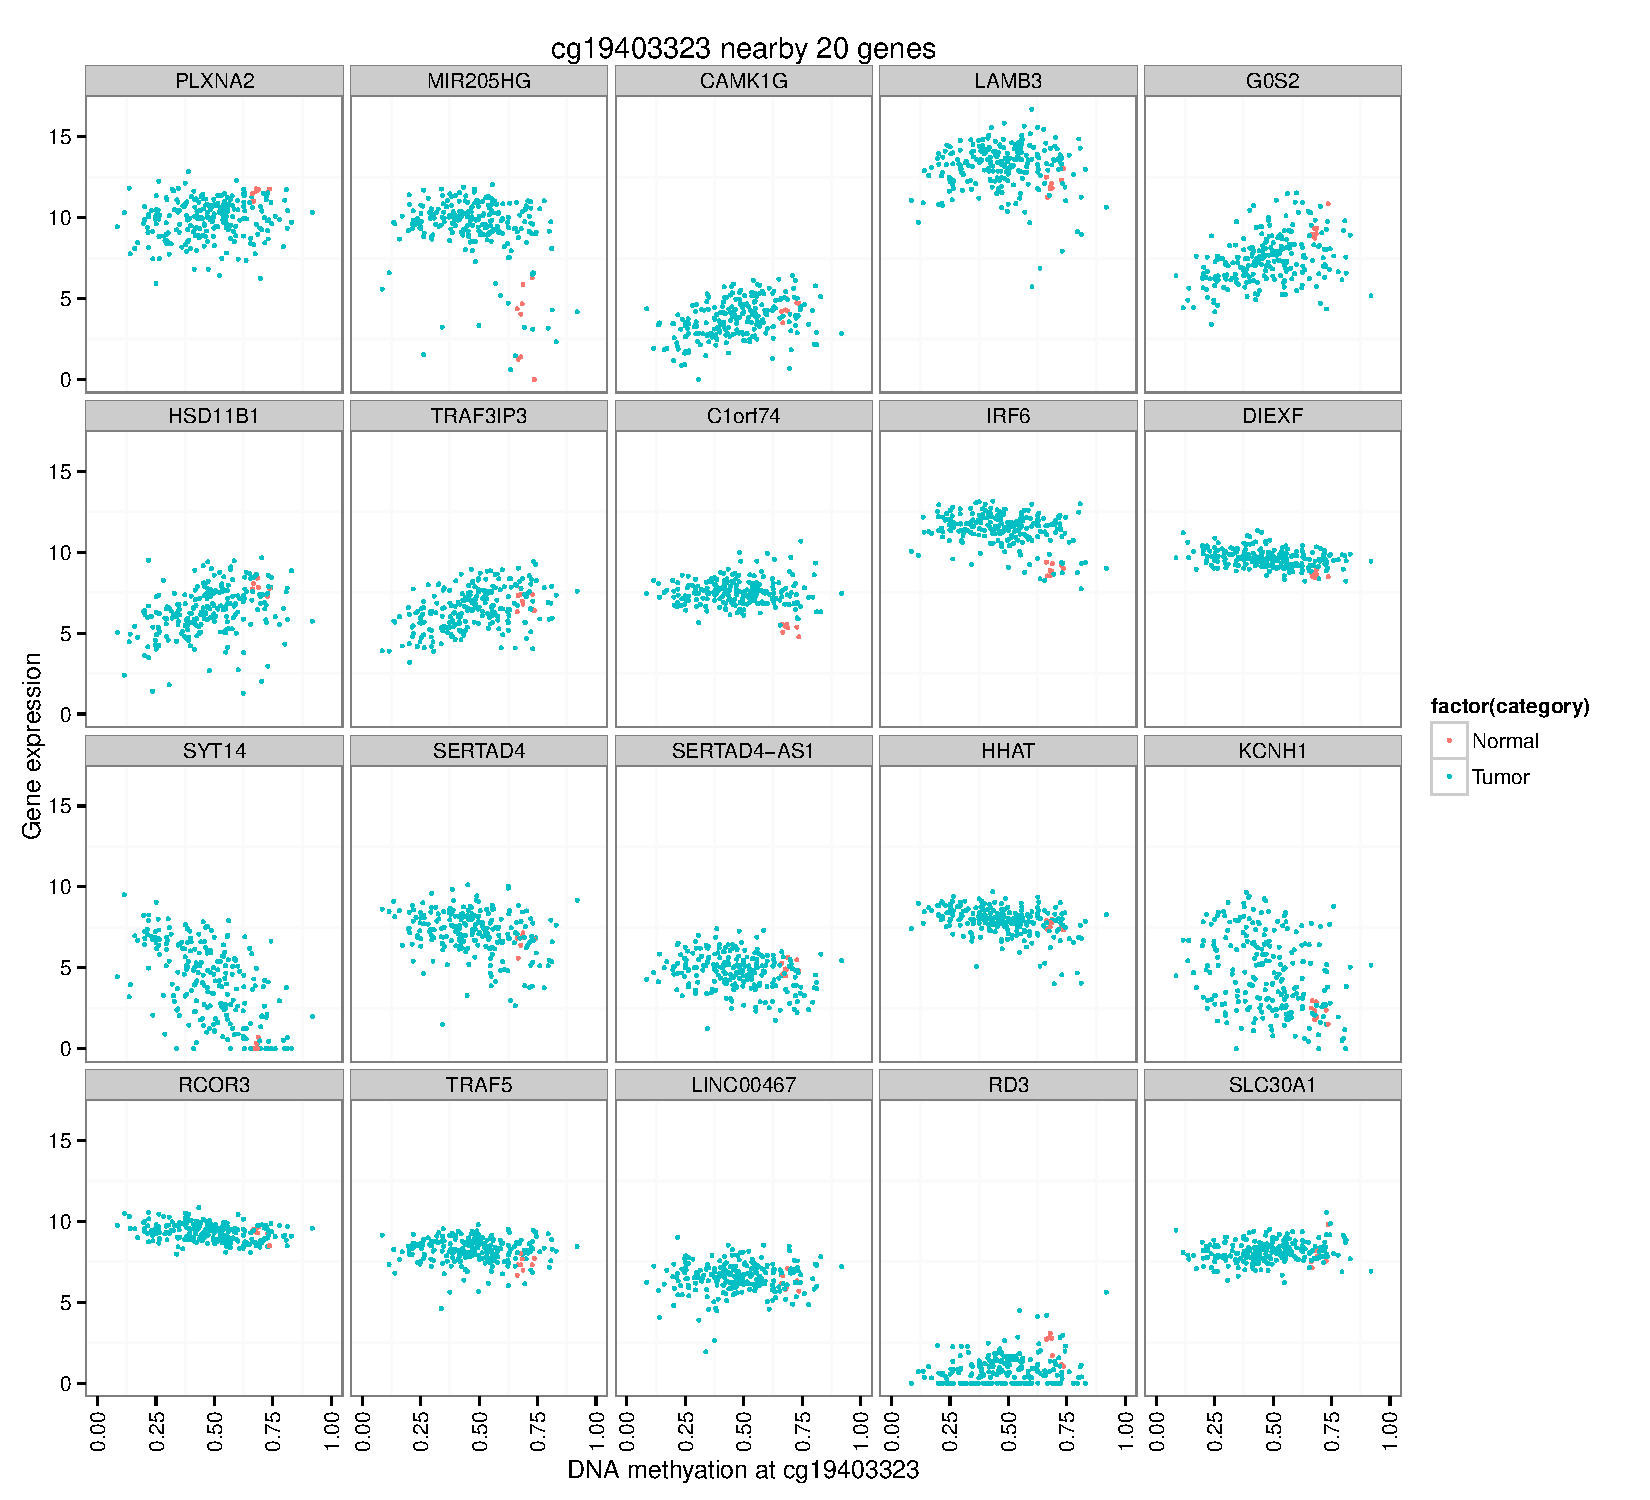
\includegraphics[width=\maxwidth]{figure/figure1-1} 

}



\end{knitrout}
\protect\caption{SEach scatter plot shows the methylation level of an example 
probe cg19403323 in all LUSC samples plotted against the expression of one of 
20 adjacent genes.
\label{fig:figure1}}
\end{figure}


\subsubsection{Scatter Plot of One Pair}
Generate a scatter plot for one probe-gene pair. Figure \ref{fig:figure2}

\begin{figure}[H]
\begin{knitrout}
\definecolor{shadecolor}{rgb}{0.969, 0.969, 0.969}\color{fgcolor}\begin{kframe}
\begin{alltt}
\hlkwd{scatter.plot}\hlstd{(mee,}\hlkwc{byPair}\hlstd{=}\hlkwd{list}\hlstd{(}\hlkwc{probe}\hlstd{=}\hlkwd{c}\hlstd{(}\hlstr{"cg19403323"}\hlstd{),}\hlkwc{gene}\hlstd{=}\hlkwd{c}\hlstd{(}\hlstr{"ID255928"}\hlstd{)),}
             \hlkwc{category}\hlstd{=}\hlstr{"TN"}\hlstd{,} \hlkwc{save}\hlstd{=}\hlnum{FALSE}\hlstd{,}\hlkwc{lm_line}\hlstd{=}\hlnum{TRUE}\hlstd{)}
\end{alltt}
\end{kframe}

{\centering 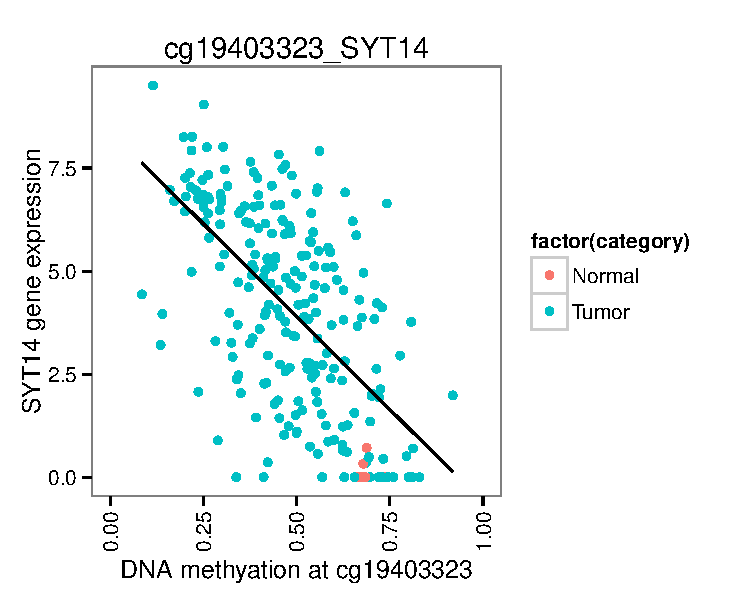
\includegraphics[width=\maxwidth]{figure/figure2-1} 

}



\end{knitrout}
\protect\caption{Scatter plot shows the methylation level of an example probe 
cg19403323 in all LUSC samples plotted against the expression of the putative 
target gene SYT14.
\label{fig:figure2}}
\end{figure}


\subsubsection{TF expression vs. average DNA methylation}
Generate scatter plot for TF expression vs average DNA methylation of the sites 
with certain motif. Figure \ref{fig:figure3}
\begin{figure}[H]
\begin{knitrout}
\definecolor{shadecolor}{rgb}{0.969, 0.969, 0.969}\color{fgcolor}\begin{kframe}
\begin{alltt}
\hlkwd{load}\hlstd{(}\hlstr{"ELMER.example/Result/LUSC/getMotif.hypo.enriched.motifs.rda"}\hlstd{)}
\hlkwd{scatter.plot}\hlstd{(mee,}\hlkwc{byTF}\hlstd{=}\hlkwd{list}\hlstd{(}\hlkwc{TF}\hlstd{=}\hlkwd{c}\hlstd{(}\hlstr{"TP53"}\hlstd{,}\hlstr{"TP63"}\hlstd{,}\hlstr{"TP73"}\hlstd{),}
             \hlkwc{probe}\hlstd{=enriched.motif[[}\hlstr{"TP53"}\hlstd{]]),} \hlkwc{category}\hlstd{=}\hlstr{"TN"}\hlstd{,}
             \hlkwc{save}\hlstd{=}\hlnum{FALSE}\hlstd{,}\hlkwc{lm_line}\hlstd{=}\hlnum{TRUE}\hlstd{)}
\end{alltt}
\end{kframe}

{\centering 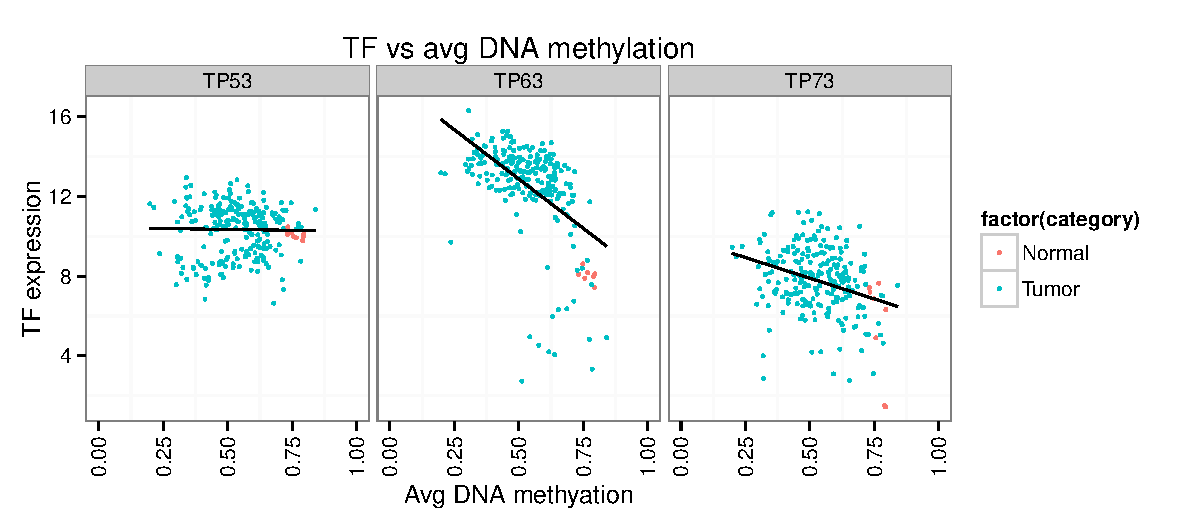
\includegraphics[width=\maxwidth]{figure/figure3-1} 

}



\end{knitrout}
\protect\caption{Each scatter plot shows the average 
methylation level of sites with the TP53 motif in all LUSC samples plotted 
against the expression of the transcription factor TP53, TP63, TP73 respectively.
\label{fig:figure3}}
\end{figure}


\subsection{Schematic plot}
Schematic plot shows a breif view of linkages between genes and probes. To make a 
schematic plot, "Pair" object should be generated first.
\begin{knitrout}
\definecolor{shadecolor}{rgb}{0.969, 0.969, 0.969}\color{fgcolor}\begin{kframe}
\begin{alltt}
\hlcom{# Make a "Pair" object for schematic.plot}
\hlstd{pair} \hlkwb{<-} \hlkwd{fetch.pair}\hlstd{(}\hlkwc{pair}\hlstd{=}\hlstr{"./ELMER.example/Result/LUSC/getPair.hypo.pairs.significant.withmotif.csv"}\hlstd{,}
                   \hlkwc{probeInfo} \hlstd{=} \hlstr{"./ELMER.example/Result/LUSC/probeInfo_feature.rda"}\hlstd{,}
                   \hlkwc{geneInfo} \hlstd{=} \hlstr{"./ELMER.example/Result/LUSC/geneAnnot.rda"}\hlstd{)}
\end{alltt}


{\ttfamily\noindent\itshape\color{messagecolor}{\#\# \textasciitilde{}\textasciitilde{}\textasciitilde{} Pair: initializator \textasciitilde{}\textasciitilde{}\textasciitilde{}}}\end{kframe}
\end{knitrout}
\newpage
\subsubsection{Nearby Genes}
Generate schematic plot for one probe with 20 nearby genes and label 
the gene significantly linked with the probe in red. Figure \ref{fig:figure4}

\begin{figure}[H]
\begin{knitrout}
\definecolor{shadecolor}{rgb}{0.969, 0.969, 0.969}\color{fgcolor}\begin{kframe}
\begin{alltt}
\hlkwd{schematic.plot}\hlstd{(}\hlkwc{pair}\hlstd{=pair,} \hlkwc{byProbe}\hlstd{=}\hlstr{"cg19403323"}\hlstd{,}\hlkwc{save}\hlstd{=}\hlnum{FALSE}\hlstd{)}
\end{alltt}


{\ttfamily\noindent\itshape\color{messagecolor}{\#\# cg19403323}}\end{kframe}

{\centering 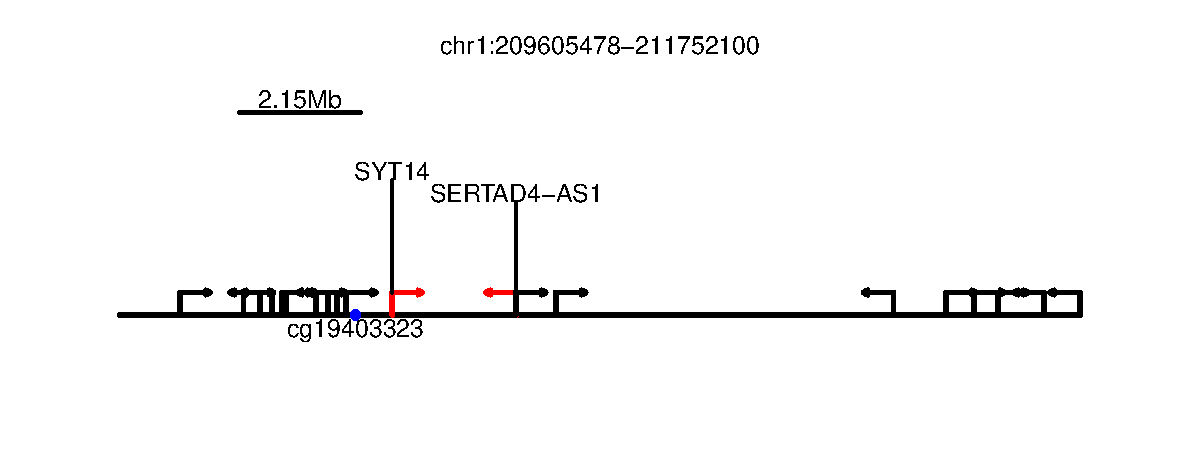
\includegraphics[width=\maxwidth]{figure/figure4-1} 

}



\end{knitrout}
\protect\caption{The schematic plot shows probe colored 
in blue and the location of nearby 20 genes. The genes significantly linked to the probe 
were shown in red.
\label{fig:figure4}}
\end{figure}


\subsubsection{Nearby Probes}
Generate schematic plot for one gene with the probes which the gene is significantly 
linked to. Figure \ref{fig:figure5}
\begin{figure}[H]
\begin{knitrout}
\definecolor{shadecolor}{rgb}{0.969, 0.969, 0.969}\color{fgcolor}\begin{kframe}
\begin{alltt}
\hlkwd{schematic.plot}\hlstd{(}\hlkwc{pair}\hlstd{=pair,} \hlkwc{byGene}\hlstd{=}\hlstr{"ID255928"}\hlstd{,}\hlkwc{save}\hlstd{=}\hlnum{FALSE}\hlstd{)}
\end{alltt}
\end{kframe}

{\centering 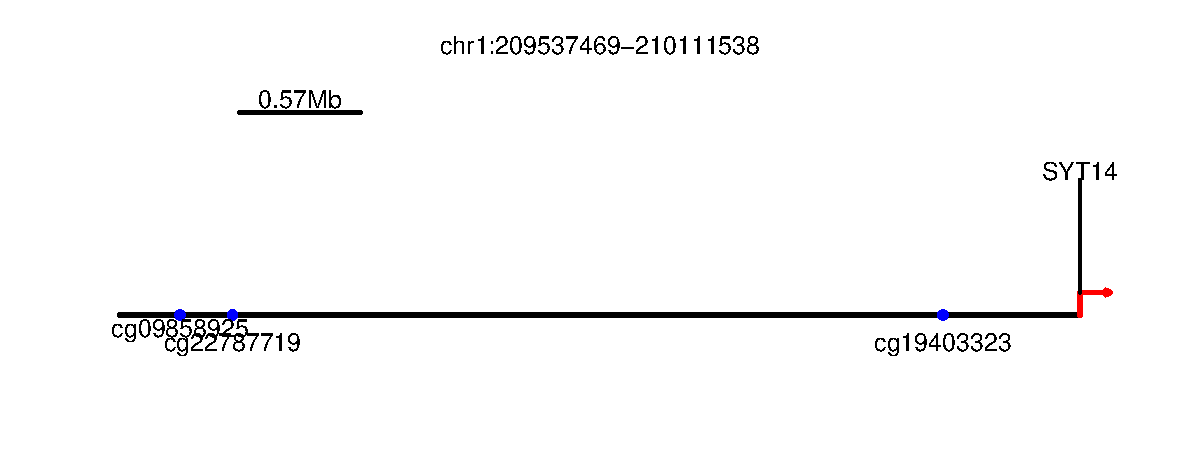
\includegraphics[width=\maxwidth]{figure/figure5-1} 

}



\end{knitrout}
\protect\caption{The schematic plot shows the gene 
colored in red and all blue colored probes, which are significantly linked to the 
expression of this gene.
\label{fig:figure5}}
\end{figure}


\subsection{Motif enrichment plot}
Motif enrichment plot shows the enrichment levels for the selected motifs. Figure\ref{fig:hypo.motif.enrichment}

\begin{figure}[H]
\begin{knitrout}
\definecolor{shadecolor}{rgb}{0.969, 0.969, 0.969}\color{fgcolor}\begin{kframe}
\begin{alltt}
\hlkwd{motif.enrichment.plot}\hlstd{(}\hlkwc{motif.enrichment}\hlstd{=}\hlstr{"./ELMER.example/Result/LUSC/getMotif.hypo.motif.enrichment.csv"}\hlstd{,}
                      \hlkwc{significant}\hlstd{=}\hlkwd{list}\hlstd{(}\hlkwc{OR}\hlstd{=}\hlnum{1.3}\hlstd{,}\hlkwc{lowerOR}\hlstd{=}\hlnum{1.3}\hlstd{),} \hlkwc{dir.out} \hlstd{=}\hlstr{"ELMER.example/Result/LUSC"}\hlstd{,}
                      \hlkwc{label}\hlstd{=}\hlstr{"hypo"}\hlstd{,} \hlkwc{save}\hlstd{=}\hlnum{FALSE}\hlstd{)}  \hlcom{## different signficant cut off.}
\end{alltt}
\end{kframe}

{\centering 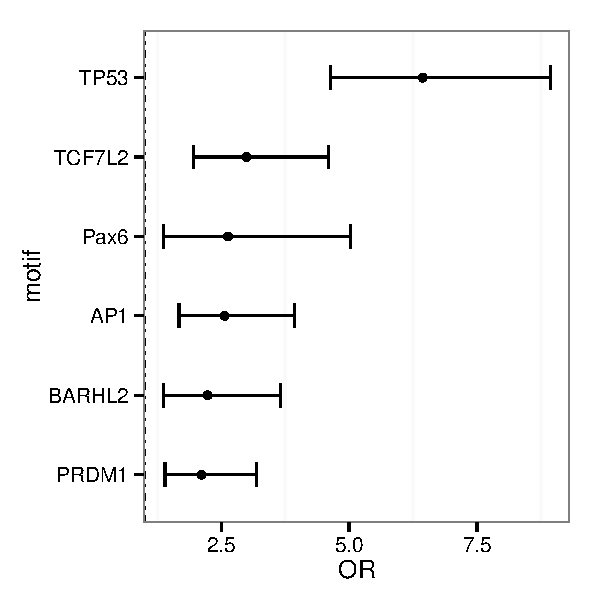
\includegraphics[width=\maxwidth]{figure/figure6-1} 

}



\end{knitrout}
\protect\caption{The plot shows the Odds Ratio (x axis) 
for the selected motifs with OR above 1.3 and lower boundary of OR above 1.3. 
The range shows the 95\% confidence interval for each Odds Ratio.
\label{fig:figure6}}
\end{figure}


\subsection{TF ranking plot}
TF ranking plot shows statistic -log10(P value) assessing the anti-correlation level 
of TFs expression level with average DNA methylation level at sites with a given motif. Figure \ref{fig:figure7}

\begin{figure}[H]
\begin{knitrout}
\definecolor{shadecolor}{rgb}{0.969, 0.969, 0.969}\color{fgcolor}\begin{kframe}
\begin{alltt}
\hlkwd{load}\hlstd{(}\hlstr{"./ELMER.example/Result/LUSC/getTF.hypo.TFs.with.motif.pvalue.rda"}\hlstd{)}
\hlkwd{TF.rank.plot}\hlstd{(}\hlkwc{motif.pvalue}\hlstd{=TF.meth.cor,} \hlkwc{motif}\hlstd{=}\hlstr{"TP53"}\hlstd{,} \hlkwc{TF.label}\hlstd{=}\hlkwd{list}\hlstd{(}\hlkwc{TP53}\hlstd{=}\hlkwd{c}\hlstd{(}\hlstr{"TP53"}\hlstd{,}\hlstr{"TP63"}\hlstd{,}\hlstr{"TP73"}\hlstd{)),}
            \hlkwc{save}\hlstd{=}\hlnum{FALSE}\hlstd{)}
\end{alltt}
\begin{verbatim}
## $TP53
\end{verbatim}
\end{kframe}

{\centering 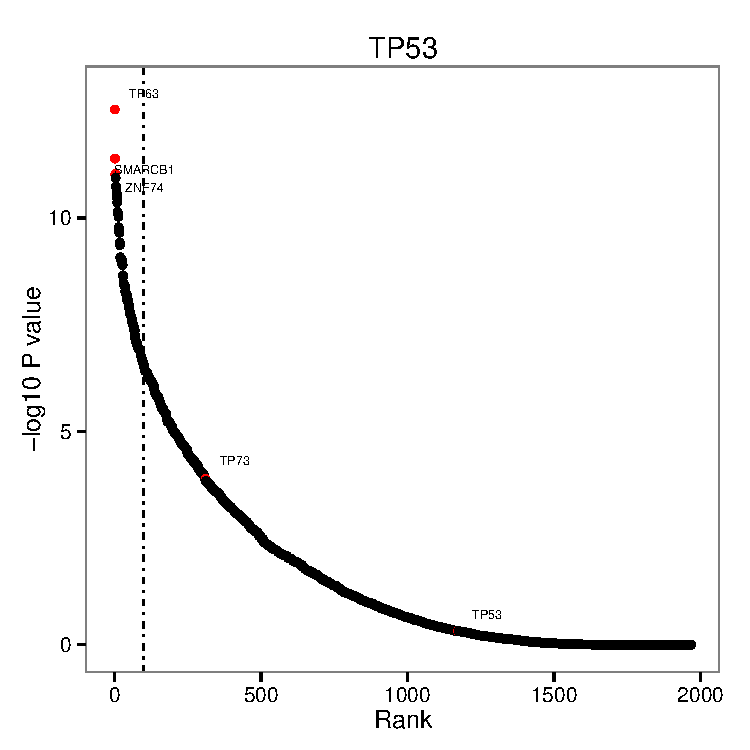
\includegraphics[width=\maxwidth]{figure/figure7-1} 

}




\end{knitrout}

\protect\caption{Shown are TF ranking plots based on 
the score (-log(P value)) of association between TF expression and DNA methylation of 
the TP53 motif in the LUSC cancer type . The dashed line indicates the boundary 
of the top 5\% association score. The top 3 associated TFs and the TF family members
(dots in red) that are associated with that specific motif are labeled in the plot.
\label{fig:figure7}}
\end{figure}

\newpage
\begin{knitrout}
\definecolor{shadecolor}{rgb}{0.969, 0.969, 0.969}\color{fgcolor}\begin{kframe}
\begin{alltt}
\hlkwd{sessionInfo}\hlstd{()}
\end{alltt}
\begin{verbatim}
## R version 3.1.2 (2014-10-31)
## Platform: x86_64-apple-darwin13.4.0 (64-bit)
## 
## locale:
## [1] en_US.UTF-8/en_US.UTF-8/en_US.UTF-8/C/en_US.UTF-8/en_US.UTF-8
## 
## attached base packages:
## [1] stats4    parallel  stats     graphics  grDevices utils     datasets  methods  
## [9] base     
## 
## other attached packages:
## [1] ELMER_0.99.4         GenomicRanges_1.18.4 GenomeInfoDb_1.2.4   IRanges_2.0.1       
## [5] S4Vectors_0.4.0      BiocGenerics_0.12.1  knitr_1.9           
## 
## loaded via a namespace (and not attached):
##  [1] BiocStyle_1.4.1  codetools_0.2-11 colorspace_1.2-6 digest_0.6.8     evaluate_0.5.5  
##  [6] formatR_1.0      ggplot2_1.0.0    grid_3.1.2       gtable_0.1.2     highr_0.4       
## [11] labeling_0.3     MASS_7.3-39      munsell_0.4.2    plyr_1.8.1       proto_0.3-10    
## [16] Rcpp_0.11.5      reshape_0.8.5    reshape2_1.4.1   scales_0.2.4     snow_0.3-13     
## [21] stringr_0.6.2    tools_3.1.2      XVector_0.6.0
\end{verbatim}
\end{kframe}
\end{knitrout}

\end{document}
